% ============================== CHAPTER 5 ===================================
\chapter{System Design}
\label{ch:design}

System design bridges the requirements of Chapter~\ref{ch:requirements} and the
implementation of Chapter~\ref{ch:implementation}. It answers the question
\emph{how}: how the system is structured, how it decomposes into modules, what
crosses the boundaries between them, how data is represented, and what the core
algorithms are.

One structural decision dominates the design and is worth stating before the
detail. \setu{} is not a single program but two programs that share a data
format. The training program is large, depends on PyTorch and Transformers, runs
on a GPU, and executes once per direction. The inference program is small,
depends only on ONNX Runtime and SentencePiece, runs on a CPU, and executes
millions of times. They meet at exactly one point: a directory containing a
quantised ONNX model and a SentencePiece tokenizer. Everything else in the
design follows from keeping that boundary clean, because it is what makes the
deployed artifact small enough and offline enough to satisfy the requirements.

\section{System Architecture}
\label{sec:architecture}

Figure~\ref{fig:sysarch} gives the high-level architecture. Data flows left to
right through four stages (corpus, distillation, training, deployment) and
then fans out to the four client interfaces.

\begin{figure}[H]
\centering
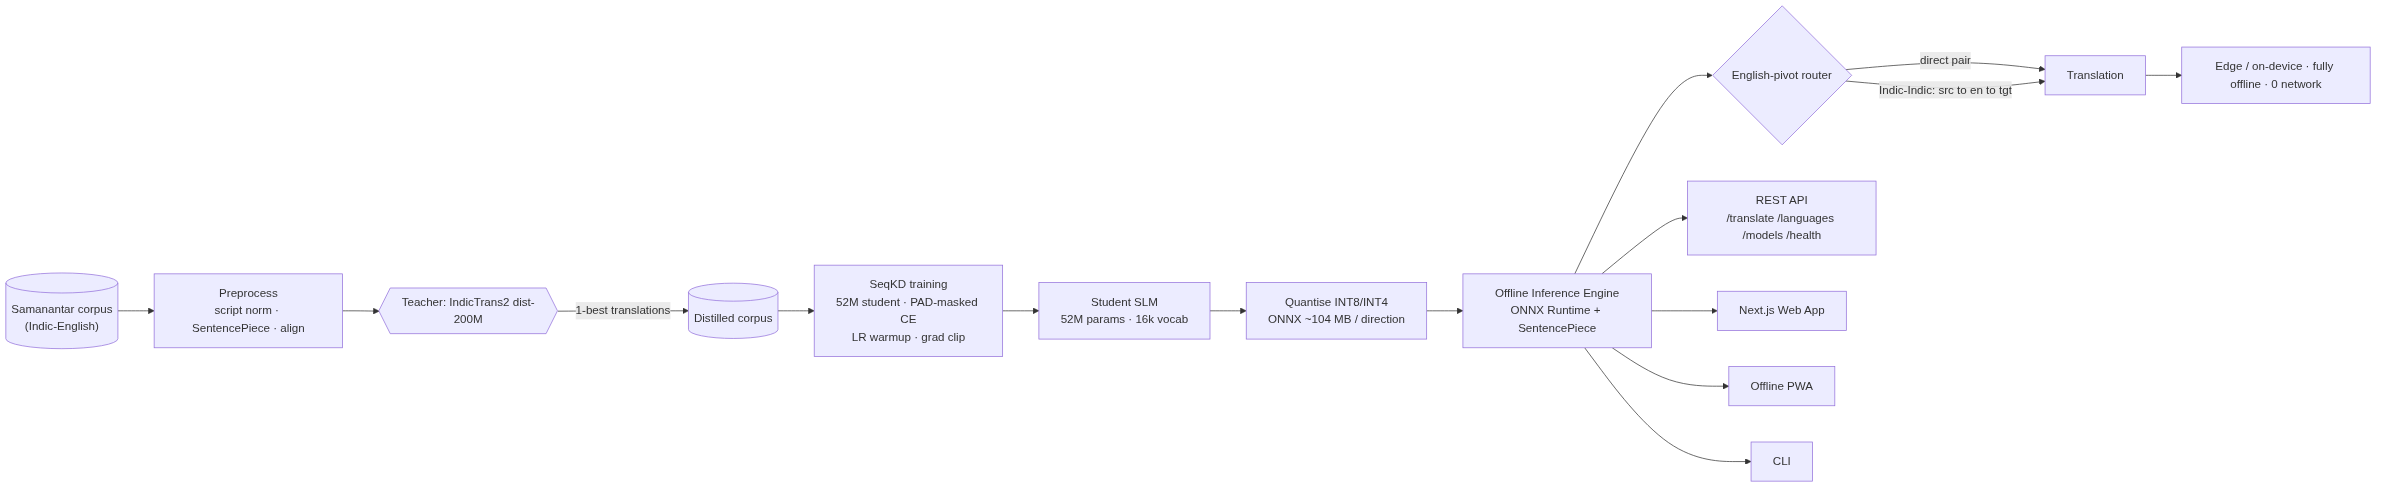
\includegraphics[width=0.99\textwidth, height=0.72\textheight, keepaspectratio]{figures/system_design.png}
\caption{System architecture: \seqkd{} distillation and offline deployment pipeline}
\label{fig:sysarch}
\end{figure}

The architecture has four layers.

\textbf{The data layer} ingests parallel corpora, normalises and filters them,
and stores two corpora per direction: the \emph{processed} corpus, which retains
human references and is used only for evaluation, and the \emph{distilled}
corpus, whose targets are the teacher's one-best translations and which is used
for training. Keeping both is what allows evaluation to remain on real
references regardless of what the student was trained on, the property that
makes the comparison in Section~\ref{sec:headtohead} fair.

\textbf{The model layer} holds the teacher behind an abstract interface and the
student behind a trainer. The teacher is used only offline, and only through
three methods. The student is a Marian encoder--decoder trained from scratch.

\textbf{The deployment layer} converts a trained student into a device artifact:
ONNX export, runtime validation, progressive INT8 and INT4 quantisation, and a
per-stage benchmark. Its output is a self-contained directory.

\textbf{The serving layer} loads those directories on demand, caches one engine
per direction, routes each request to a direct model or through the English
pivot, and presents the result through four interfaces that share the routing
code exactly.

\subsection{Design Principles}
\label{subsec:principles}

Five principles were applied consistently and explain most of the specific
choices that follow.

\textbf{One direction, one model.} Each translation direction gets its own
student. This avoids the cross-lingual interference that multilingual
distillation frameworks report \cite{ref:aiokd}, permits an independent quality
gate per direction, and means a collapsed direction can be retrained without
disturbing any other. The cost is storage, 104\,MB per direction, which the
English pivot then bounds at $2n$ rather than $n^2$.

\textbf{The teacher lives behind a wall.} \texttt{IndicTrans2Teacher} is the only
module permitted to import \texttt{transformers}, \texttt{torch} or
\texttt{IndicTransToolkit}. A unit test walks the source tree and fails the
build on any violation. This is what guarantees that the inference path carries
no training dependencies.

\textbf{Configuration, not code.} The language pair, model dimensions,
hyperparameters, corpus sources and cleaning thresholds all live in YAML.
Adding a language is a configuration change and a data fetch. A dedicated test
verifies that the pipeline is pair-agnostic by running it on a different pair
end to end.

\textbf{Fail loudly, never silently.} When no model exists for a requested pair
the engine returns the input unchanged but sets \texttt{stub: true}, so a caller
can never mistake a passthrough for a translation. When the scorecard has no
evidence for a target it prints \textsc{unverified} rather than a pass. This
principle is why the 0.796 ratio in an early report was printed as a failure
rather than rounded up.

\textbf{Resumability by construction.} Every pipeline stage writes a completion
marker. A multi-hour run interrupted by a disconnection resumes at the stage it
reached, which matters because teacher distillation over 500{,}000 sentences is
too expensive to repeat.

\section{Component Design / Module Decomposition}
\label{sec:modules}

The system decomposes into eight modules. Each has a single responsibility, a
defined input and output, and its own tests.

\subsection{Module 1: Corpus Loader}
\label{subsec:mod1}

\textbf{Responsibility:} turn a raw parallel corpus into a clean, deduplicated
set of \texttt{CorpusEntry} objects.

The module streams Samanantar from Hugging Face (streaming rather than
downloading, because the full corpus is tens of gigabytes and only a slice is
needed) and passes each pair through four stages. \emph{Normalisation}
applies Unicode NFC and strips control characters while explicitly preserving
zero-width joiners and non-joiners, which carry meaning in Indic scripts.
\emph{Filtering} removes pairs shorter than 3 or longer than 1024 characters,
pairs whose source-to-target length ratio exceeds 3.0 (a reliable signal of
misalignment in mined data), and pairs in which fewer than half the letters
belong to the expected script. \emph{Deduplication} removes exact duplicates.
\emph{Reporting} records how many pairs each filter removed.

A representative run illustrates the module's value: 50{,}000 input pairs
yielded 49{,}520 clean pairs, with 253 removed for length ratio, 213 for wrong
script, 10 for excessive length and 4 as duplicates. Roughly one pair in a
hundred of web-mined data is unusable, and the wrong-script filter in particular
catches pairs where one side is simply not in the language it claims to be.

\subsection{Module 2: Teacher Distiller}
\label{subsec:mod2}

\textbf{Responsibility:} replace every human reference target with the teacher's
own one-best translation of the source.

\texttt{SeqKDDistiller} batches source sentences, calls the teacher's
\texttt{generate\_candidates\_batch} with $n=1$, and emits new
\texttt{CorpusEntry} objects tagged \texttt{seqkd}. Greedy decoding is used
rather than beam search: it is four to five times faster, which is what makes
distilling half a million sentences feasible within a session, and the resulting
targets are of equivalent utility for training.

The module degrades safely. If the teacher returns an empty candidate for some
sentence, the original human reference is retained for that pair and the event
is counted in the module's statistics, so a teacher hiccup cannot silently
introduce blank training targets.

\subsection{Module 3: \seqkd{} Trainer}
\label{subsec:mod3}

\textbf{Responsibility:} train a 52.6-million-parameter student from scratch on
the distilled corpus.

The trainer implements token-level cross-entropy with five components, each
added in response to an observed failure rather than adopted by convention:

\begin{itemize}
  \item \textbf{PAD masking.} Label positions corresponding to padding are set
        to $-100$ so that the loss ignores them. Before this fix the model
        received free credit for predicting padding, which produced a
        fake-low loss of 0.274 and a decoder that ignored the source entirely.
  \item \textbf{Linear warmup and decay.} The warmup length is capped at
        10\,\% of the run. A from-scratch Transformer trained at a constant
        learning rate underfits badly; the configuration option existed but was
        being silently ignored.
  \item \textbf{Label smoothing (0.1) and dropout (0.2).} Standard regularisers
        against overconfidence and memorisation.
  \item \textbf{Gradient-norm clipping at 1.0.} The single most important
        stabiliser. Without it, a 200{,}000-sentence run collapsed to a constant
        output while the identical code at 120{,}000 sentences had succeeded: more steps simply meant more opportunities to hit a gradient spike.
  \item \textbf{Generation safeguards.} Decoding suppresses the PAD, UNK and BOS
        tokens and forbids repeated 3-grams, so output can never be empty and
        cannot degenerate into a repeated phrase.
\end{itemize}

The module also implements DPO with a frozen supervised-fine-tuning reference
model. A test enforces that the reference model's parameters never receive
gradients, since an unfrozen reference silently reduces DPO to a no-op. This
path is retained for the reported comparison but is not used for the shipped
models.

\subsection{Module 4: Quantiser}
\label{subsec:mod4}

\textbf{Responsibility:} convert a trained PyTorch checkpoint into a deployable
ONNX artifact.

The module exports to FP32 ONNX, validates the export by running it through ONNX
Runtime and comparing outputs, then quantises progressively (INT8 first, INT4
second), benchmarking size and latency at each stage. The measured progression
for a 52.6-million-parameter student is 410.9\,MB FP32, 104.6\,MB INT8 and
103.9\,MB INT4.

The near-identity of the INT8 and INT4 sizes is an honest limitation rather than
a measurement error: the ONNX Runtime CPU execution provider has no true 4-bit
kernel, so INT4 export falls back to 8-bit storage for most tensors. The INT4
variant is nonetheless the one shipped, because it benchmarked marginally faster
and, in several directions, marginally more accurate.

\subsection{Module 5: Inference Engine and Pivot Router}
\label{subsec:mod5}

\textbf{Responsibility:} translate text using a quantised student, offline, and
route requests to the right student.

\texttt{InferenceEngine} loads an ONNX session and a local SentencePiece
tokenizer, encodes the source, decodes greedily, and returns a
\texttt{TranslationResult} carrying the translated text and the measured
latency. An \texttt{assert\_offline()} helper disables all sockets to prove that
inference needs no network.

The router sits above it and solves the coverage problem. Given a source and
target language it resolves both to FLORES codes, rejects identical pairs and
unknown codes, then checks for a directly trained model. If one exists it
translates in a single hop. If not (the case for every Indic-to-Indic pair,
since no ungated Indic-to-Indic teacher was available), it checks whether both
source\arrowto{}English and English\arrowto{}target models exist, and if so
chains them, returning the combined latency and a \texttt{pivot: "en"} flag. The
arithmetic is favourable: 22 direct models serve 132 usable directions, and
measured two-hop latency is approximately 50--65\,ms.

Engines are cached one per pair, so a direction is loaded from disk at most
once, and every interface calls this single router rather than reimplementing
routing. Consolidating the routing logic here fixed a real defect: the CLI had
previously constructed an engine with the default configured pair, so
\texttt{-{}-src as} silently translated using the Hindi model.

\subsection{Module 6: REST API}
\label{subsec:mod6}

\textbf{Responsibility:} expose the engine over HTTP.

A FastAPI service provides four endpoints. \texttt{POST /translate} accepts a
source language, target language and text and returns the translation with
latency and pivot information. \texttt{GET /languages} returns the registry of
22 scheduled languages plus English, marking which are trained. \texttt{GET
/models} scans the models directory and reports every discovered pair with its
quantisation variant and size on disk. \texttt{GET /health} reports readiness.
CORS is enabled so that a browser client can call the service directly.

\subsection{Module 7: Client Interfaces}
\label{subsec:mod7}

\textbf{Responsibility:} make the engine usable.

Four clients share the engine. The \textbf{CLI} accepts text from an argument, a
file or standard input and emits plain text or JSON. The \textbf{Next.js web
client} provides a translator console with source and target pickers, a swap
control, live latency display and an on-device indicator; all 23 languages
appear in the picker, with the trained ones grouped as available and the
remainder shown but disabled, so coverage is visible rather than hidden. The
\textbf{offline progressive web application} caches its shell through a service
worker and continues to function without a network. \textbf{Mobile SDK stubs}
for Android and iOS wrap the same API surface.

\subsection{Module 8: Evaluator and Expansion Mechanisms}
\label{subsec:mod8}

\textbf{Responsibility:} measure quality, and provide a route to adding
languages.

The evaluator computes BLEU and chrF with sacreBLEU on a held-out slice of real
human references, computes the teacher's score on the identical slice, and
reports the ratio. Loaders for FLORES-200 and IN22 are implemented for
benchmark-grade numbers, along with COMET scoring and paired-bootstrap
significance testing.

Two expansion mechanisms are implemented and tested. \textbf{All-in-One
knowledge distillation} trains one student across several directions with
temperature-sampled cross-lingual balancing and a coverage report; a sampling
temperature above 1.0 flattens the distribution towards uniform and so protects
low-resource directions from being swamped. \textbf{Elastic Weight
Consolidation} adds a diagonal-Fisher penalty that anchors parameters important
to previously learned languages, enabling a new language to be added without a
full retrain. Its tests prove the penalty is zero at the snapshot point, grows
with distance from it, and (measured rather than assumed) keeps
Fisher-weighted drift on an old task below that of plain fine-tuning after a
conflicting new task.

\section{Interface Design}
\label{sec:interface}

\subsection{External Interfaces}
\label{subsec:extinterface}

\begin{longtable}{@{}L{2.5cm} L{4.2cm} L{7.4cm}@{}}
\caption{External interface specification}
\label{tab:interfaces}\\
\toprule
\rowcolor{headblue}
\textbf{Component} & \textbf{Description} & \textbf{Details and example} \\
\midrule
\endfirsthead
\toprule
\rowcolor{headblue}
\textbf{Component} & \textbf{Description} & \textbf{Details and example} \\
\midrule
\endhead
\bottomrule
\endlastfoot

REST: translate & Primary translation endpoint & \texttt{POST /translate} with body \texttt{\{source\_lang, target\_lang, text\}}; returns \texttt{\{translated\_text, latency\_ms, pivot, stub\}}. Example request: \texttt{\{"source\_lang":"hi", "target\_lang":"en", "text":"..."\}} \\
\rowcolor{rowgrey}
REST: languages & Language registry & \texttt{GET /languages} $\rightarrow$ 22 scheduled languages plus English, each with ISO code, FLORES code, script and endonym \\
REST: models & Model discovery & \texttt{GET /models} $\rightarrow$ \texttt{\{"count": 22, "models": [\{pair, variant, size\_mb\}, ...]\}} \\
\rowcolor{rowgrey}
REST: health & Readiness probe & \texttt{GET /health} $\rightarrow$ \texttt{\{"status":"ok", "stub": false\}} \\
CLI & Command-line translation & \texttt{python setu\_cli.py -{}-src hi -{}-tgt en -{}-text "..."}; also \texttt{-{}-file} and standard input, with \texttt{-{}-json} output \\
\rowcolor{rowgrey}
Web client & Browser translator console & Language pickers grouped into available and not-yet-trained, swap control, live latency, on-device badge, curated Indic-to-Indic examples \\
Offline PWA & Installable offline client & Service-worker shell caching; functions with no network after first load \\
\rowcolor{rowgrey}
Mobile SDK & Android and iOS wrapper & \texttt{translate(text, srcLang, tgtLang)} over the same engine \\
Training CLI & Pipeline entry points & \texttt{setu-data}, \texttt{setu-distill}, \texttt{setu-quantize}, \texttt{setu-eval}, \texttt{setu-report}, and \texttt{scripts/train\_full.py} \\

\end{longtable}

\subsection{User Interface Design}
\label{subsec:uidesign}

The web client was designed around one principle: a user must be able to tell,
at a glance, whether a translation was produced on their device and how good the
coverage is for their language. Three affordances implement it.

The \textbf{on-device badge} reports whether the response came from a real
quantised model or the passthrough stub, alongside the measured latency in
milliseconds. A user is never shown a number without knowing what produced it.

The \textbf{language picker} lists all 23 languages, not only the trained ones.
Trained languages are grouped under an ``available now'' heading; the remaining
eleven appear below, visibly disabled and labelled as Phase 2. Hiding untrained
languages would have made the system look complete; showing them disabled makes
the actual coverage legible.

The \textbf{pivot indicator} tells the user when a translation was routed
through English, because a two-hop translation has different failure
characteristics from a single-hop one and the user is entitled to know.

Visually the client uses a warm paper-and-ink palette with a single accent
colour, a light and dark theme, and typography that names every language in its
own script (\dev{हिन्दी}, \ben{বাংলা}, \tam{தமிழ்}, \tel{తెలుగు},
\kan{ಕನ್ನಡ}, \mal{മലയാളം}, \guj{ગુજરાતી}, \ory{ଓଡ଼ିଆ}, \gur{ਪੰਜਾਬੀ}) rather
than transliterating them into Latin. Fonts are self-hosted so that the client
loads no external resource at run time, which is a functional requirement rather
than a stylistic one.

\section{Data Structure Design}
\label{sec:datastructures}

Four data objects carry all information between modules. Their field names are
stable across the entire codebase, which is what allows modules to be developed
and tested independently.

\begin{table}[H]
\centering
\caption{Core data structures}
\label{tab:datastructures}
\begin{tabular}{@{}L{3.6cm} L{4.2cm} L{6.3cm}@{}}
\toprule
\rowcolor{headblue}
\textbf{Structure} & \textbf{Fields} & \textbf{Purpose} \\
\midrule
\texttt{CorpusEntry} & \texttt{src\_lang}, \texttt{tgt\_lang}, \texttt{src\_text}, \texttt{tgt\_text}, \texttt{source} & One parallel sentence pair. The \texttt{source} tag distinguishes a human reference from a \texttt{seqkd} teacher target, so the two corpora never mix \\
\rowcolor{rowgrey}
\texttt{PreferencePair} & \texttt{src\_text}, \texttt{preferred\_tgt}, \texttt{dispreferred\_tgt}, \texttt{quality\_delta} & One DPO training example. \texttt{quality\_delta} is the chrF gap; pairs below a threshold are discarded as too noisy to teach from \\
\texttt{ModelConfig} & \texttt{language\_pair}, \texttt{params}, \texttt{quantization} & Full student specification: architecture, layer counts, hidden size, vocabulary size, sequence length, quantisation mode \\
\rowcolor{rowgrey}
\texttt{TranslationResult} & \texttt{translated\_text}, \texttt{src\_lang}, \texttt{tgt\_lang}, \texttt{latency\_ms}, \texttt{pivot} & One translation with its provenance. \texttt{pivot} is \texttt{None} for direct translation and \texttt{"en"} for a chained one \\
\bottomrule
\end{tabular}
\end{table}

\subsection{On-Disk Layout}
\label{subsec:ondisk}

Corpora are stored as JSONL, one entry per line, which streams without loading
the whole file and appends cheaply. Reports are JSON. A deployed model
directory is self-contained:

\begin{verbatim}
models/<src_flores>-<tgt_flores>/
  |-- int4/       encoder + decoder ONNX (103.9 MB, shipped)
  |-- int8/       the INT8 variant (104.6 MB)
  |-- onnx/       the FP32 export (410.9 MB, not shipped)
  |-- tokenizer/  SentencePiece model and vocabulary
  `-- quantize_report.json    per-stage size and latency
\end{verbatim}

Model discovery scans for exactly this layout, which is why dropping a trained
model directory into place is all that is needed for the API to serve it.

\subsection{The Tokenizer's Reserved Tags}
\label{subsec:tokenizer}

The SentencePiece vocabulary is 16{,}000 unigram tokens, chosen after a
32{,}000-token vocabulary was measured to leave most tokens undertrained on the
available data and to produce degenerate decoding. All 23 FLORES language tags
are reserved as special tokens from the very first training run, even for
languages not yet trained. This costs 23 vocabulary slots and buys a guarantee:
token identifiers do not shift when a language is added, so previously trained
models remain valid and no re-tokenisation is ever required.

\section{Algorithm Design}
\label{sec:algorithms}

\subsection{Algorithm 1: Sequence-Level Knowledge Distillation}
\label{subsec:alg1}

This is the core training algorithm and the one the empirical comparison
selected.

\begin{longtable}{@{}L{14.0cm}@{}}
\caption{Algorithm 1: \seqkd{} training of one direction}
\label{tab:alg1}\\
\toprule
\rowcolor{headblue}
\textbf{Input:} cleaned corpus $C = \{(x_i, y_i)\}_{i=1}^{N}$; teacher $T$; student architecture $\theta$ \\
\rowcolor{headblue}
\textbf{Output:} trained student parameters $\theta^{*}$ \\
\midrule
\endfirsthead
\multicolumn{1}{c}{\textit{Table \thetable{} (continued)}}\\
\toprule
\rowcolor{headblue}
\textbf{Input:} cleaned corpus $C = \{(x_i, y_i)\}_{i=1}^{N}$; teacher $T$; student architecture $\theta$ \\
\rowcolor{headblue}
\textbf{Output:} trained student parameters $\theta^{*}$ \\
\midrule
\endhead
\midrule
\multicolumn{1}{r}{\textit{continued on next page}}\\
\endfoot
\bottomrule
\endlastfoot

\textbf{1.} \textbf{for} each batch $B \subseteq C$ \textbf{do} \\
\textbf{2.} \quad $\hat{y}_i \leftarrow T.\textsc{decode}(x_i)$ \quad \textit{// greedy one-best; discard the human $y_i$} \\
\textbf{3.} \quad \textbf{if} $\hat{y}_i$ is empty \textbf{then} $\hat{y}_i \leftarrow y_i$ \quad \textit{// safe fallback, counted} \\
\textbf{4.} \quad append $(x_i, \hat{y}_i)$ to the distilled corpus $D$ \\
\textbf{5.} \textbf{end for} \\
\textbf{6.} initialise $\theta$ randomly; initialise AdamW with linear warmup then decay \\
\textbf{7.} \textbf{for} epoch $= 1 \ldots E$ \textbf{do} \\
\textbf{8.} \quad \textbf{for} each batch $(x, \hat{y}) \subseteq D$ \textbf{do} \\
\textbf{9.} \quad\quad $\ell \leftarrow \textsc{CrossEntropy}(\theta(x), \hat{y})$ with pad labels set to $-100$ and label smoothing $0.1$ \\
\textbf{10.} \quad\quad backpropagate; $\textsc{ClipGradNorm}(\theta, 1.0)$; optimiser step; scheduler step \\
\textbf{11.} \quad \textbf{end for} \\
\textbf{12.} \quad evaluate on held-out \emph{human} references; record BLEU, chrF and the teacher ratio \\
\textbf{13.} \textbf{end for} \\
\textbf{14.} \textbf{return} $\theta^{*}$ \\
\end{longtable}

Three details carry the algorithm's correctness. Line~2 discards the human
target; that is the whole method, and it is what breaks the reference-noise
ceiling. Line~9's $-100$ masking is what keeps the loss honest. Line~12
evaluates on human references even though training used teacher targets, which
is what makes the numbers comparable with a reference-trained baseline.

\subsection{Algorithm 2: English-Pivot Routing}
\label{subsec:alg2}

\begin{longtable}{@{}L{14.0cm}@{}}
\caption{Algorithm 2: routing a translation request}
\label{tab:alg2}\\
\toprule
\rowcolor{headblue}
\textbf{Input:} text $t$; source language $s$; target language $g$ \\
\rowcolor{headblue}
\textbf{Output:} translation, pivot flag, stub flag \\
\midrule
\endfirsthead
\multicolumn{1}{c}{\textit{Table \thetable{} (continued)}}\\
\toprule
\rowcolor{headblue}
\textbf{Input:} text $t$; source language $s$; target language $g$ \\
\rowcolor{headblue}
\textbf{Output:} translation, pivot flag, stub flag \\
\midrule
\endhead
\midrule
\multicolumn{1}{r}{\textit{continued on next page}}\\
\endfoot
\bottomrule
\endlastfoot

\textbf{1.} $s \leftarrow \textsc{ResolveFlores}(s)$; \ $g \leftarrow \textsc{ResolveFlores}(g)$ \quad \textit{// raises on an unknown code} \\
\textbf{2.} \textbf{if} $s = g$ \textbf{then raise} \textsc{ValueError} \quad \textit{// identical source and target} \\
\textbf{3.} $d \leftarrow$ \texttt{"}$s$\texttt{-}$g$\texttt{"} \\
\textbf{4.} \textbf{if} \textsc{ModelExists}($d$) \textbf{then return} $(\textsc{Engine}(d).\textsc{translate}(t),\ \textsc{None},\ \textsc{False})$ \\
\textbf{5.} \textbf{if} $s \neq$ \texttt{eng\_Latn} \textbf{and} $g \neq$ \texttt{eng\_Latn} \textbf{then} \\
\textbf{6.} \quad $h_1 \leftarrow$ \texttt{"}$s$\texttt{-eng\_Latn"}; \ $h_2 \leftarrow$ \texttt{"eng\_Latn-}$g$\texttt{"} \\
\textbf{7.} \quad \textbf{if} \textsc{ModelExists}($h_1$) \textbf{and} \textsc{ModelExists}($h_2$) \textbf{then} \\
\textbf{8.} \quad\quad $r_1 \leftarrow \textsc{Engine}(h_1).\textsc{translate}(t)$ \quad \textit{// source to English} \\
\textbf{9.} \quad\quad $r_2 \leftarrow \textsc{Engine}(h_2).\textsc{translate}(r_1.\text{text})$ \quad \textit{// English to target} \\
\textbf{10.} \quad\quad \textbf{return} $(r_2 \text{ with latency } r_1.\text{ms} + r_2.\text{ms},\ \texttt{"en"},\ \textsc{False})$ \\
\textbf{11.} \quad \textbf{end if} \\
\textbf{12.} \textbf{end if} \\
\textbf{13.} \textbf{return} $(t,\ \textsc{None},\ \textsc{True})$ \quad \textit{// passthrough, explicitly flagged as a stub} \\
\end{longtable}

Engines are memoised per pair, so the model-existence checks on lines 4 and 7
are cheap after the first call. Line~13 is the honesty guarantee: when nothing
can translate the request the input is returned unchanged and explicitly marked,
never presented as a translation.

\subsection{Algorithm 3: Progressive Quantisation}
\label{subsec:alg3}

\begin{table}[H]
\centering
\caption{Algorithm 3: export and progressive quantisation}
\label{tab:alg3}
\begin{tabular}{@{}L{14.0cm}@{}}
\toprule
\rowcolor{headblue}
\textbf{Input:} trained checkpoint $\theta^{*}$; benchmark sentence set $S$ \\
\rowcolor{headblue}
\textbf{Output:} INT8 and INT4 ONNX artifacts with a size and latency report \\
\midrule
\textbf{1.} export $\theta^{*}$ to FP32 ONNX; \textbf{assert} the checkpoint path exists (fail clearly, not as a remote identifier) \\
\textbf{2.} validate: run the ONNX graph through ONNX Runtime and compare against the PyTorch output \\
\textbf{3.} $m_{32} \leftarrow \textsc{SizeMB}$; \ $(p_{50}, p_{90}, p_{\max}) \leftarrow \textsc{Benchmark}(S)$ \\
\textbf{4.} apply dynamic INT8 quantisation; re-measure size and latency \\
\textbf{5.} apply INT4 quantisation; re-measure size and latency \\
\textbf{6.} \textbf{for} each variant \textbf{do assert} $\text{size} \leq 200$\,MB \textbf{and} $p_{90} < 500$\,ms \\
\textbf{7.} verify translation succeeds with all network sockets disabled \\
\textbf{8.} write \texttt{quantize\_report.json}; package the chosen variant with its tokenizer \\
\bottomrule
\end{tabular}
\end{table}

\subsection{Algorithm 4: Preference Pair Generation (Reported Baseline)}
\label{subsec:alg4}

This algorithm produced the DPO training data for the comparison in
Section~\ref{sec:headtohead}. It is retained in the system and documented here
because the negative result it supports is one of the project's findings, but it
is not used for the shipped models.

\begin{table}[H]
\centering
\caption{Algorithm 4: chrF-ranked preference pair construction}
\label{tab:alg4}
\begin{tabular}{@{}L{14.0cm}@{}}
\toprule
\rowcolor{headblue}
\textbf{Input:} corpus entries; teacher $T$; candidate count $n$; neighbour count $k$; minimum delta $\delta$ \\
\rowcolor{headblue}
\textbf{Output:} validated \texttt{PreferencePair} list \\
\midrule
\textbf{1.} \textbf{for} each entry $(x, y)$ \textbf{do} \\
\textbf{2.} \quad $A \leftarrow T.\textsc{generateCandidates}(x, n)$ \quad \textit{// beam search, $n$ returned sequences} \\
\textbf{3.} \quad $A \leftarrow A \cup \textsc{KnnNeighbourTranslations}(x, k)$ \quad \textit{// char n-gram TF-IDF retrieval} \\
\textbf{4.} \quad score every $a \in A$ by sentence chrF against the human reference $y$ \\
\textbf{5.} \quad $a^{+} \leftarrow \arg\max_a \textsc{chrF}(a, y)$ \\
\textbf{6.} \quad \textbf{for} each $a^{-} \in A \setminus \{a^{+}\}$ \textbf{do} \\
\textbf{7.} \quad\quad $\Delta \leftarrow \textsc{chrF}(a^{+}, y) - \textsc{chrF}(a^{-}, y)$ \\
\textbf{8.} \quad\quad \textbf{if} $\Delta \geq \delta$ \textbf{then} emit $(x, a^{+}, a^{-}, \Delta)$ \quad \textit{// otherwise too noisy to teach from} \\
\textbf{9.} \quad \textbf{end for} \\
\textbf{10.} \textbf{end for} \\
\textbf{11.} \textbf{assert} $\textsc{chrF}(a^{+}) > \textsc{chrF}(a^{-})$ for every emitted pair \quad \textit{// validation gate} \\
\bottomrule
\end{tabular}
\end{table}

A representative run turned 500 corpus entries into 3{,}494 candidates and
2{,}074 validated pairs, discarding 920 for insufficient quality delta; the
delta distribution had a median of 31.3 chrF points. On GPU the same pipeline
produced 33{,}535 validated pairs from 8{,}000 entries. The preference data is
therefore plentiful and well separated, which is precisely why the negative
result is informative. DPO trained on this data reaches a margin accuracy of
1.0, ranking every preferred candidate above its dispreferred counterpart, and
still does not improve translation quality over sequence-level distillation.
